\chapter{Einleitung}

\section{Motivation}
Ziel des Versuchs ist die Bestimmung der spezifischen Wärmekapazität verschiedener Festkörper (Graphit, Aluminium, Blei) in zwei Temperaturbereichen.  
Im ersten Versuchsteil wird die Wärmekapazität im Bereich von etwa \SI{20}{\celsius} bis \SI{100}{\celsius} mithilfe eines Wasserkalorimeters bestimmt.  
Im zweiten Versuchsteil wird die Wärmekapazität bei tiefen Temperaturen zwischen Raumtemperatur und \SI{-195.8}{\celsius} (Temperatur von flüssigem Stickstoff) ermittelt.  

Die Untersuchung erlaubt es, sowohl den klassischen Bereich, in dem die Dulong-Petitsche Regel eine Näherung darstellt, als auch den nieder­temperatur­bereich zu erfassen, in dem quantenmechanische Effekte dominieren. Auf diese Weise wird die Temperaturabhängigkeit der Wärmekapazität sichtbar, und es lässt sich auch eine Abschätzung der Debye-Temperatur der Materialien vornehmen.

\section{Physikalische Grundlagen}
\cite{skript25}
\subsection*{Definitionen}
Führt man einem Körper eine Wärme \( Q \) zu, so erhöht sich seine Temperatur um
\begin{equation}
    C = \frac{Q}{\Delta T}
    \label{eq:waermekapazitaet}
\end{equation}
mit der Wärmekapazität \( C \).  

Die spezifische Wärmekapazität und die molare Wärmekapazität lauten:
\begin{equation}
    c = \frac{Q}{m \Delta T},
    \label{eq:spezifische_waermekapazitaet}
\end{equation}
\begin{equation}
    c_{\text{mol}} = \frac{M}{m}\frac{Q}{\Delta T}.
    \label{eq:molwaerme}
\end{equation}

\subsection*{Mischungsmethode im Kalorimeter}
Ein Festkörper der Temperatur \(T_1\) wird in ein Kalorimeter mit Wasser der Temperatur \(T_2\) getaucht. Die Mischungstemperatur sei \(T\). Die abgegebene Wärme des Festkörpers:
\begin{equation}
    Q = m_x c_x (T_1 - T)
    \label{eq:waerme_festkoerper}
\end{equation}
entspricht der vom Wasser und Kalorimeter aufgenommenen Wärme:
\begin{equation}
    Q = (m_w c_w + W)(T - T_2).
    \label{eq:waerme_wasser}
\end{equation}
Durch Umstellen ergibt sich die gesuchte Größe:
\begin{equation}
    c_x = \frac{(m_w c_w + W)(T - T_2)}{m_x (T_1 - T)}.
    \label{eq:spezifische_kalorimeter}
\end{equation}

Zur Bestimmung des Wasserwerts \( W \):
\begin{equation}
    W = m_w c_w \frac{T_1 - T}{T - T_2}, \qquad T_1 > T_2.
    \label{eq:wasserwert}
\end{equation}

\subsection*{Bestimmung mit flüssigem Stickstoff}
Taucht man einen Festkörper der Temperatur \(T_1\) in flüssigen Stickstoff mit \(T_2 \approx \SI{-195.8}{\celsius}\), so gilt:
\begin{equation}
    Q = m_x c_x (T_1 - T_2).
    \label{eq:stickstoff_waerme}
\end{equation}
Die Wärme wird zum Verdampfen des Stickstoffs genutzt:
\begin{equation}
    Q = Q_V m_V,
    \label{eq:verdampfungswaerme}
\end{equation}
mit der Verdampfungswärme \( Q_V = \SI{199}{\joule\per\gram} \). Kombination von Gleichungen \hyperref[eq:stickstoff_waerme]{\ref*{eq:stickstoff_waerme}} und \hyperref[eq:verdampfungswaerme]{\ref*{eq:verdampfungswaerme}} liefert:
\begin{equation}
    c_x = \frac{Q_V m_V}{m_x (T_1 - T_2)}.
    \label{eq:stickstoff_cx}
\end{equation}

\subsection*{Theoretische Modelle}
Nach dem Äquipartitionsprinzip besitzt jeder Freiheitsgrad die Energie
\begin{equation}
    \langle E \rangle = k_B T.
    \label{eq:aquipartition}
\end{equation}
Für ein Mol Atome folgt:
\begin{equation}
    U_{\text{mol}} = 3 N_A k_B T = 3 R T.
    \label{eq:energie_mol}
\end{equation}
Daraus ergibt sich die Dulong-Petitsche Regel:
\begin{equation}
    c_V \approx 3R.
    \label{eq:dulong_petit}
\end{equation}
Diese Näherung gilt nur eingeschränkt. Genauere Ergebnisse liefert das Debye-Modell, welches die quantisierten Gitterschwingungen berücksichtigt und die Debye-Temperatur \(\Theta_D\) als charakteristische Größe einführt.

\begin{figure}[h!]
    \centering
    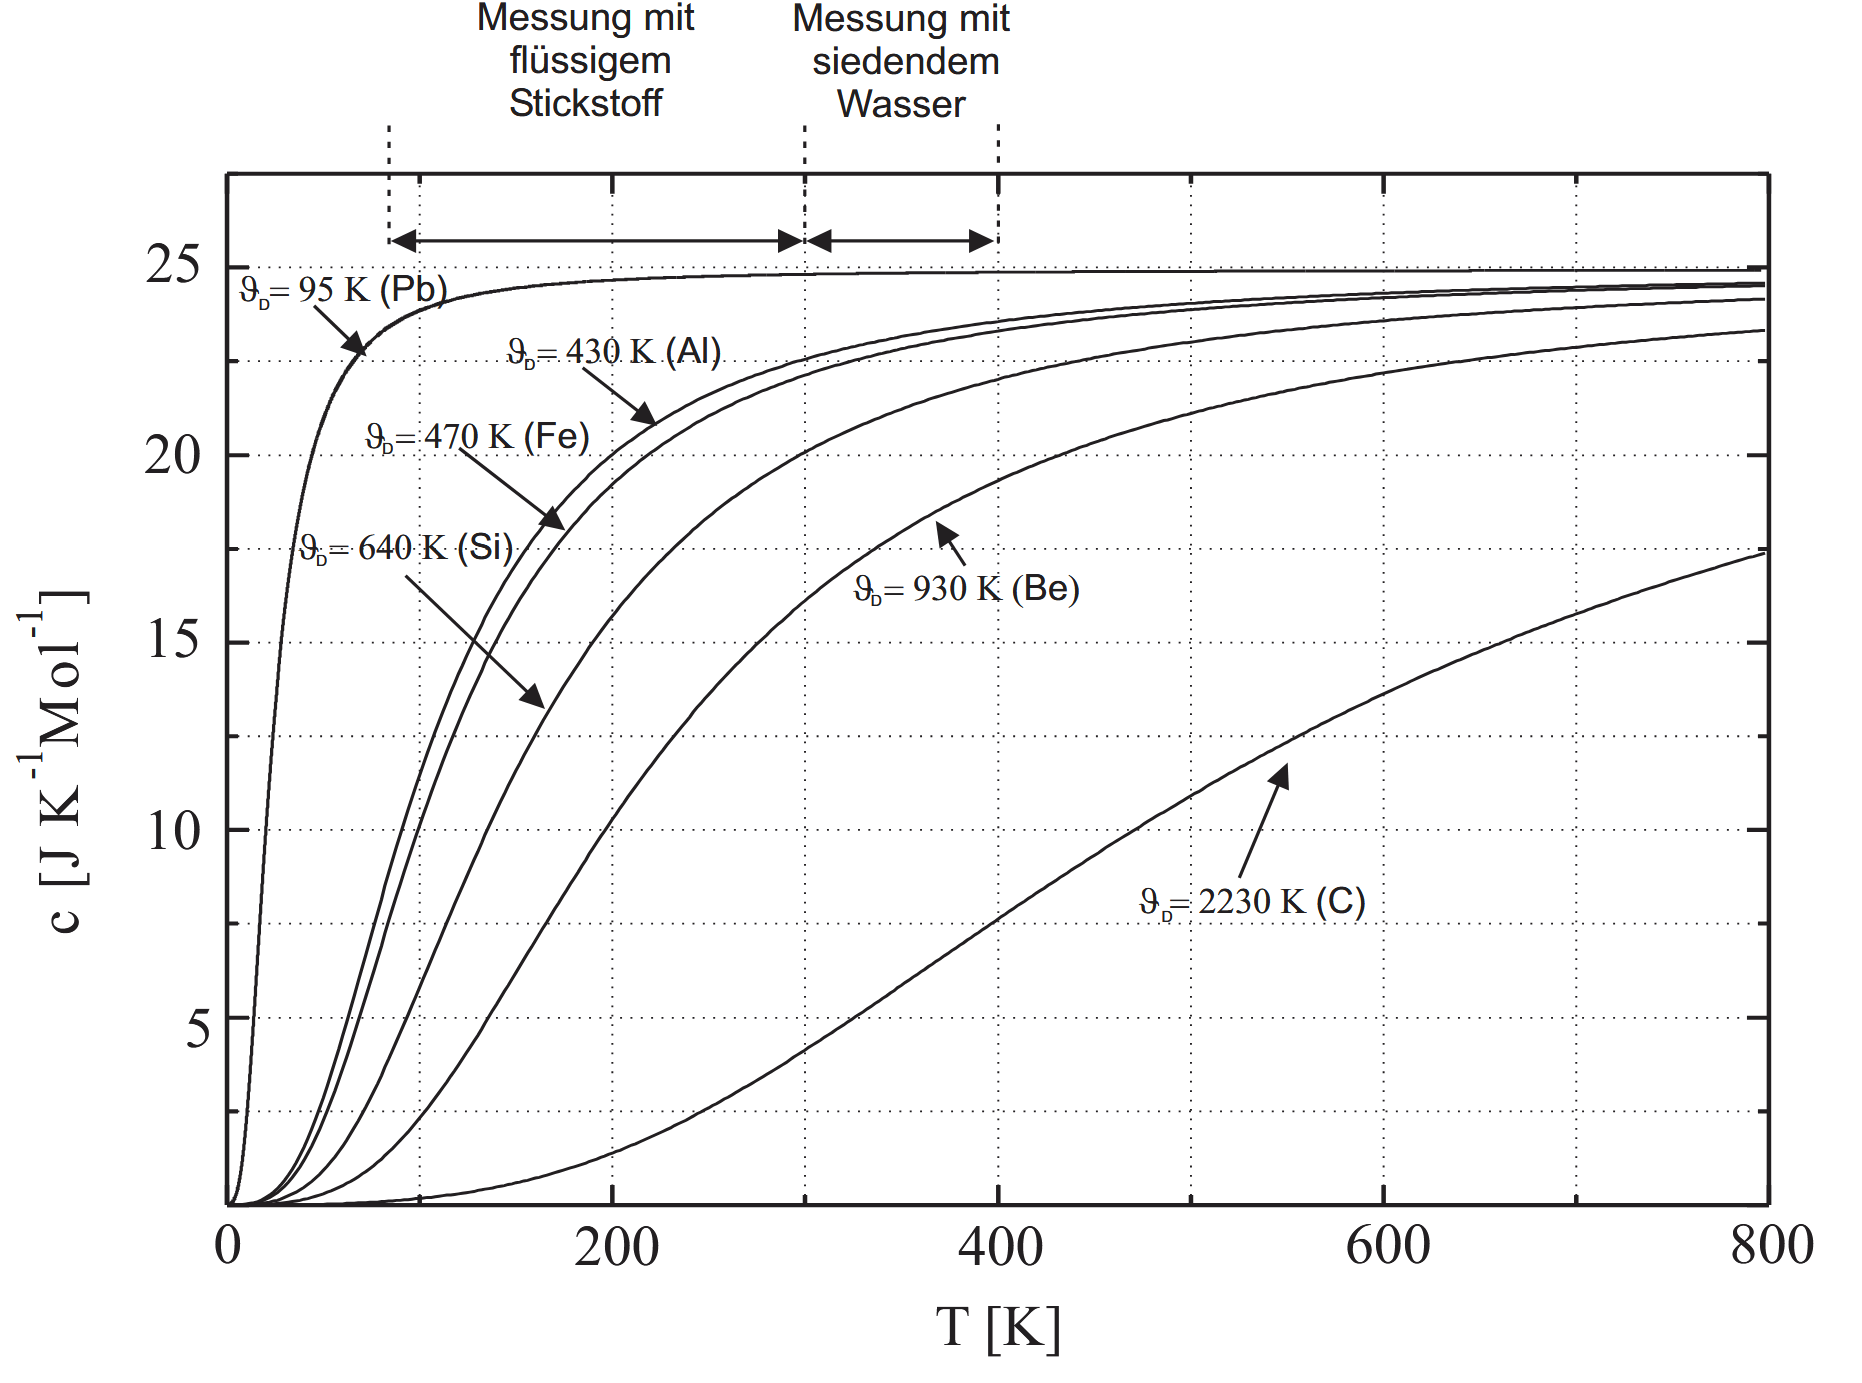
\includegraphics[width=0.5\textwidth]{img/\versuchsnummer/Debye-Modell.png}
    \caption{Debye-Modell}
    \label{img:de_mod}
\end{figure}
